% Chapter 6: Sprint 3 - File Management & Geolocation Tracking

\chapter{Sprint 3: File Management and Geolocation Tracking}

\section{Introduction}

Sprint 3 extends the core intervention management system with file management capabilities and geolocation tracking. This sprint enables technicians to capture and upload photographic evidence, attach documents, and track intervention location data. The implementation provides secure file storage and location-aware intervention tracking.

The sprint delivers critical functionality for evidence management, allowing supervisors and clients to access comprehensive documentation of completed interventions. Geolocation tracking provides accountability and operational insights into technician activities and intervention execution locations.

\section{Sprint Preview and Objectives}

\subsection{User Stories}

\begin{enumerate}
\item \textbf{US-S3-001: File Upload and Management}
  \begin{itemize}
  \item \textbf{As a} technician
  \item \textbf{I want} to attach photos and documents to interventions
  \item \textbf{So that} I can provide evidence of work completion
  \item \textbf{Story Points:} 13
  \end{itemize}

\item \textbf{US-S3-002: Geolocation Tracking}
  \begin{itemize}
  \item \textbf{As a} system
  \item \textbf{I want} to capture technician location during interventions
  \item \textbf{So that} supervisors can verify work locations and track movements
  \item \textbf{Story Points:} 8
  \end{itemize}

\item \textbf{US-S3-003: File Download and Sharing}
  \begin{itemize}
  \item \textbf{As a} supervisor
  \item \textbf{I want} to download and share intervention files with clients
  \item \textbf{So that} clients can access evidence and documentation
  \item \textbf{Story Points:} 8
  \end{itemize}

\item \textbf{US-S3-004: Image Compression and Optimization}
  \begin{itemize}
  \item \textbf{As a} system
  \item \textbf{I want} to compress and optimize uploaded images
  \item \textbf{So that} storage space is used efficiently and downloads are fast
  \item \textbf{Story Points:} 8
  \end{itemize}
\end{enumerate}
\subsection{Sprint Goals}

\begin{enumerate}
\item \textbf{File Management:} Implement secure file upload, storage, and retrieval with access control
\item \textbf{Location Services:} Integrate GPS tracking with intervention data capture
\item \textbf{Evidence Management:} Enable supervisors to manage and share intervention evidence
\end{enumerate}

\section{Sprint Backlog}

The 45-point sprint focuses on file operations and location tracking:

\begin{table}[H]
\centering
\caption{Sprint 3 Backlog}
\label{tab:sprint3_backlog}
\begin{tabularx}{\textwidth}{|l|X|l|l|}
\hline
\textbf{ID} & \textbf{User Story} & \textbf{Points} & \textbf{Status} \\
\hline
S3-1 & File upload and management & 13 & Completed \\
\hline
S3-2 & Geolocation tracking & 8 & Completed \\
\hline
S3-3 & File download and sharing & 8 & Completed \\
\hline
S3-4 & Image compression & 8 & Completed \\
\hline
\textbf{Total} & & \textbf{37} & \\
\hline
\end{tabularx}
\end{table}

\section{Functional Specification}

\subsection{Use Cases}

\textbf{UC-FILE-001: Upload Intervention File}
\begin{itemize}
\item \textbf{Primary Actor:} Technician
\item \textbf{Main Success Scenario:}
  \begin{enumerate}
  \item Technician selects intervention
  \item Technician attaches file (photo, document)
  \item System validates file type and size
  \item System compresses image if applicable
  \item System uploads file to storage
  \item System links file to intervention
  \item Technician receives upload confirmation
  \end{enumerate}
\end{itemize}

\textbf{UC-GPS-001: Capture Location Data}
\begin{itemize}
\item \textbf{Primary Actor:} Mobile Application
\item \textbf{Main Success Scenario:}
  \begin{enumerate}
  \item Technician opens intervention
  \item System requests location permission
  \item System captures GPS coordinates
  \item System records timestamp
  \item Technician completes intervention
  \item System stores location with intervention data
  \end{enumerate}
\end{itemize}

\section{Conception}

\subsection{Use Diagram}

\begin{figure}[H]
\centering
\fbox{\parbox{1\textwidth}{
\centering
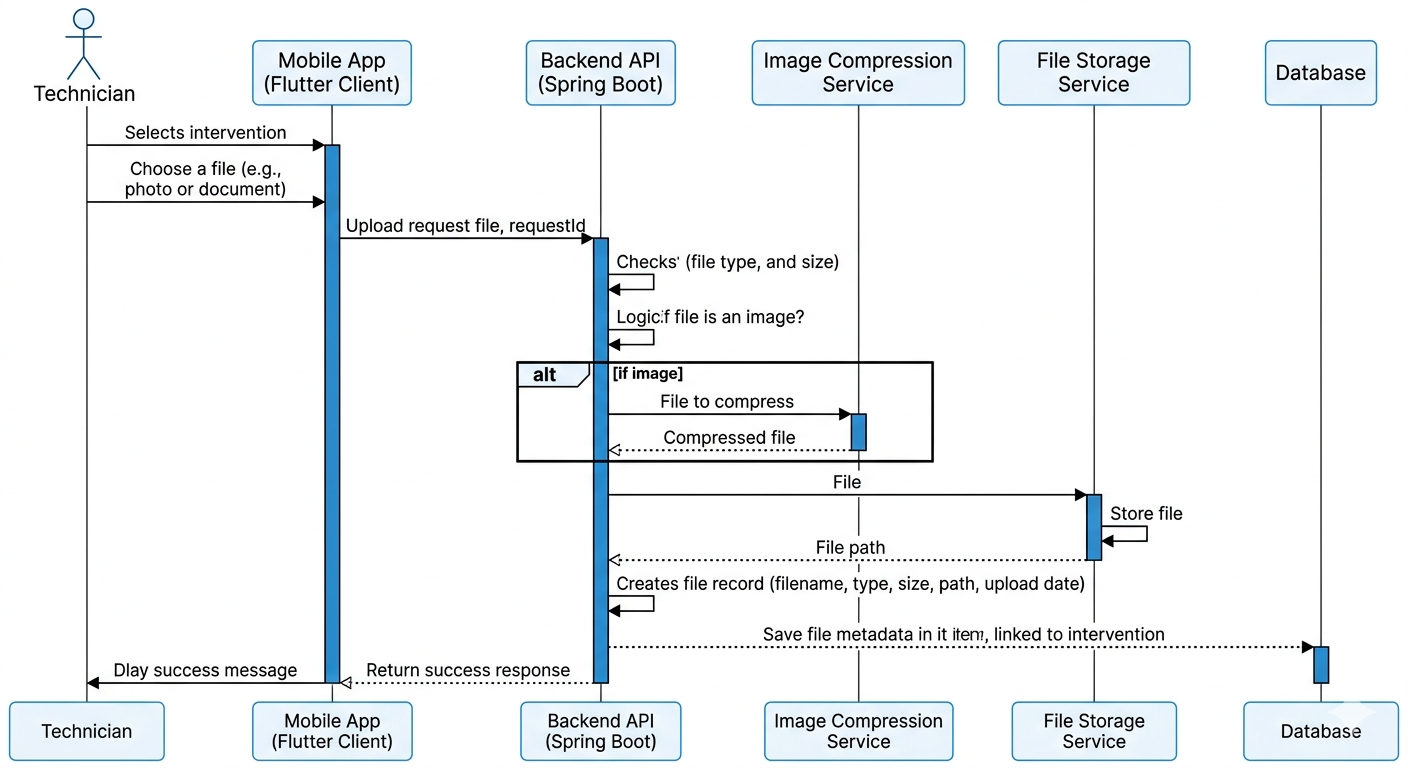
\includegraphics[width=1\textwidth]{seqFile.png} 
Sequence diagram illustrating the file upload and management process during Sprint 3.
}}
\caption{Sprint 3 File Upload and Management Sequence}
\label{fig:sprint3_sequence_file}
\end{figure}

\section{Realization}

\subsection{Backend Implementation Details}

The backend implementation in Sprint 3 focused on extending the intervention domain with file management and geolocation tracking capabilities.

\begin{itemize}
\item Secure file upload and storage with metadata persistence
\item Image compression and optimization before storage
\item File-to-intervention association management
\item Geolocation data capture and persistence linked to intervention execution
\item Access control for file retrieval and download operations
\end{itemize}

File management is handled through a dedicated service layer responsible for validating file size and type, applying compression for image files, and delegating storage to the file system or storage provider. Each uploaded file is persisted with metadata including filename, type, size, and storage path, and is linked to a specific intervention request.

Geolocation tracking is integrated into the execution workflow by associating latitude, longitude, and timestamps with each intervention. This enables traceability of technician activities and verification of intervention locations.

Primary endpoint groups delivered:

\begin{itemize}
\item \api{files}
\item \api{files/download}
\item \api{execution-details}
\end{itemize}

\subsection{Frontend Implementation}

The Angular web application was extended to support file management and evidence visualization features for supervisors and coordinators.

\begin{itemize}
\item File listing interface within intervention details view
\item Download and preview functionality for uploaded documents and images
\item Integration of evidence files into intervention tracking screens
\item Visualization of geolocation data associated with interventions
\end{itemize}

The UI enables users to access all files attached to an intervention, download them securely, and share them with external stakeholders. Location data is displayed in a structured format, allowing supervisors to verify execution locations.

\begin{figure}[H]
\centering
\fbox{\parbox{1\textwidth}{
\centering
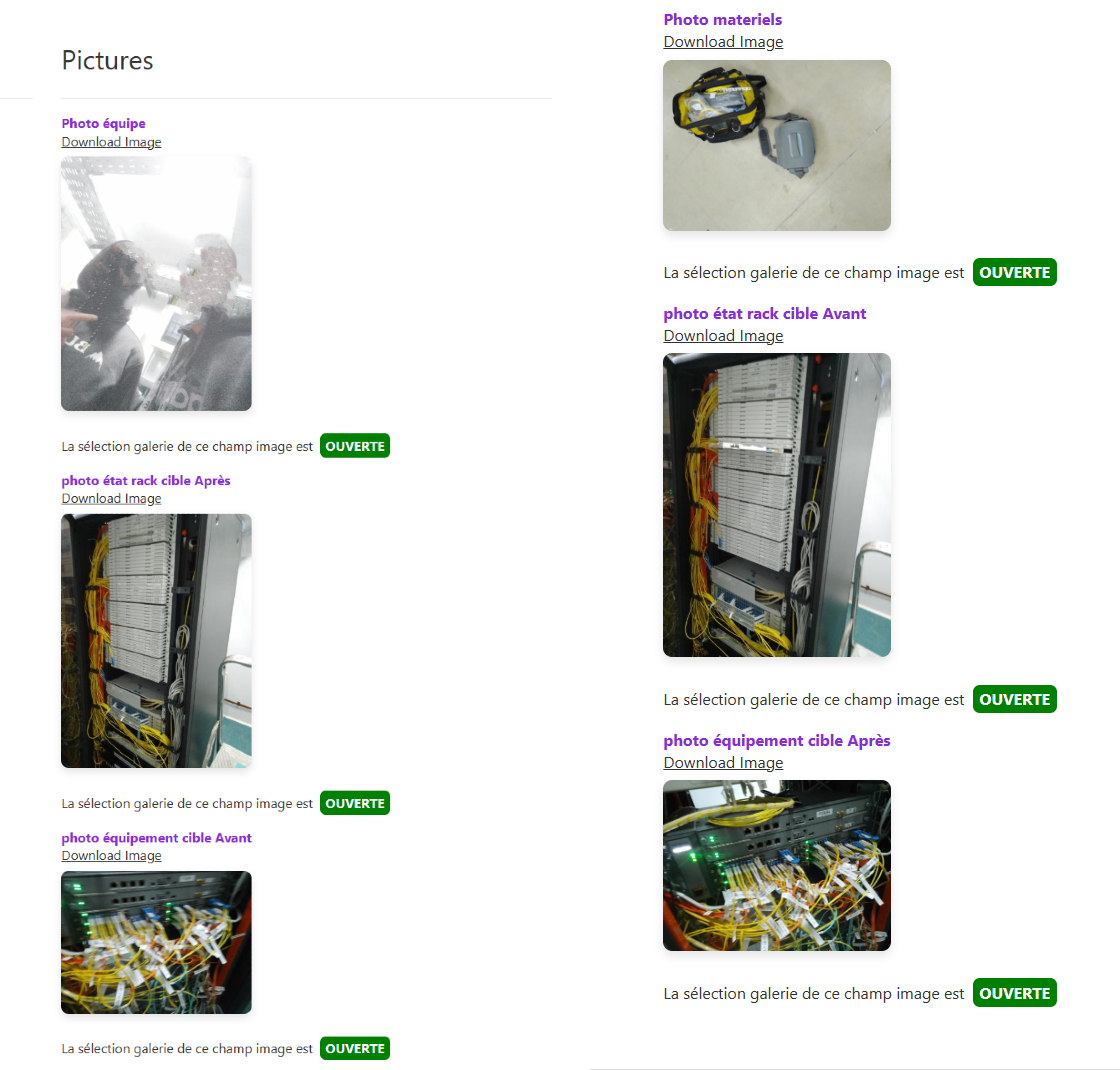
\includegraphics[width=1\textwidth]{fnial.png}
Angular UI : Intervention evidence management with file listing, download, and preview.
}}
\caption{Sprint 3 Angular UI - File Management}
\label{fig:sprint3_angular_files}
\end{figure}

\subsection{Mobile Implementation }

The Flutter mobile application was enhanced to support real-time file capture and geolocation tracking during intervention execution.

\begin{itemize}
\item Capture and upload of images and documents from device storage or camera
\item Client-side image compression before upload
\item Integration of file upload within intervention workflow
\item GPS location capture with permission handling
\item Association of location data with intervention execution
\end{itemize}

The mobile application ensures efficient data transfer by compressing images before upload and provides fallback handling for connectivity issues. Geolocation services are integrated to capture accurate position data during intervention execution.

\begin{figure}[H]
\centering
\fbox{\parbox{1\textwidth}{
\centering
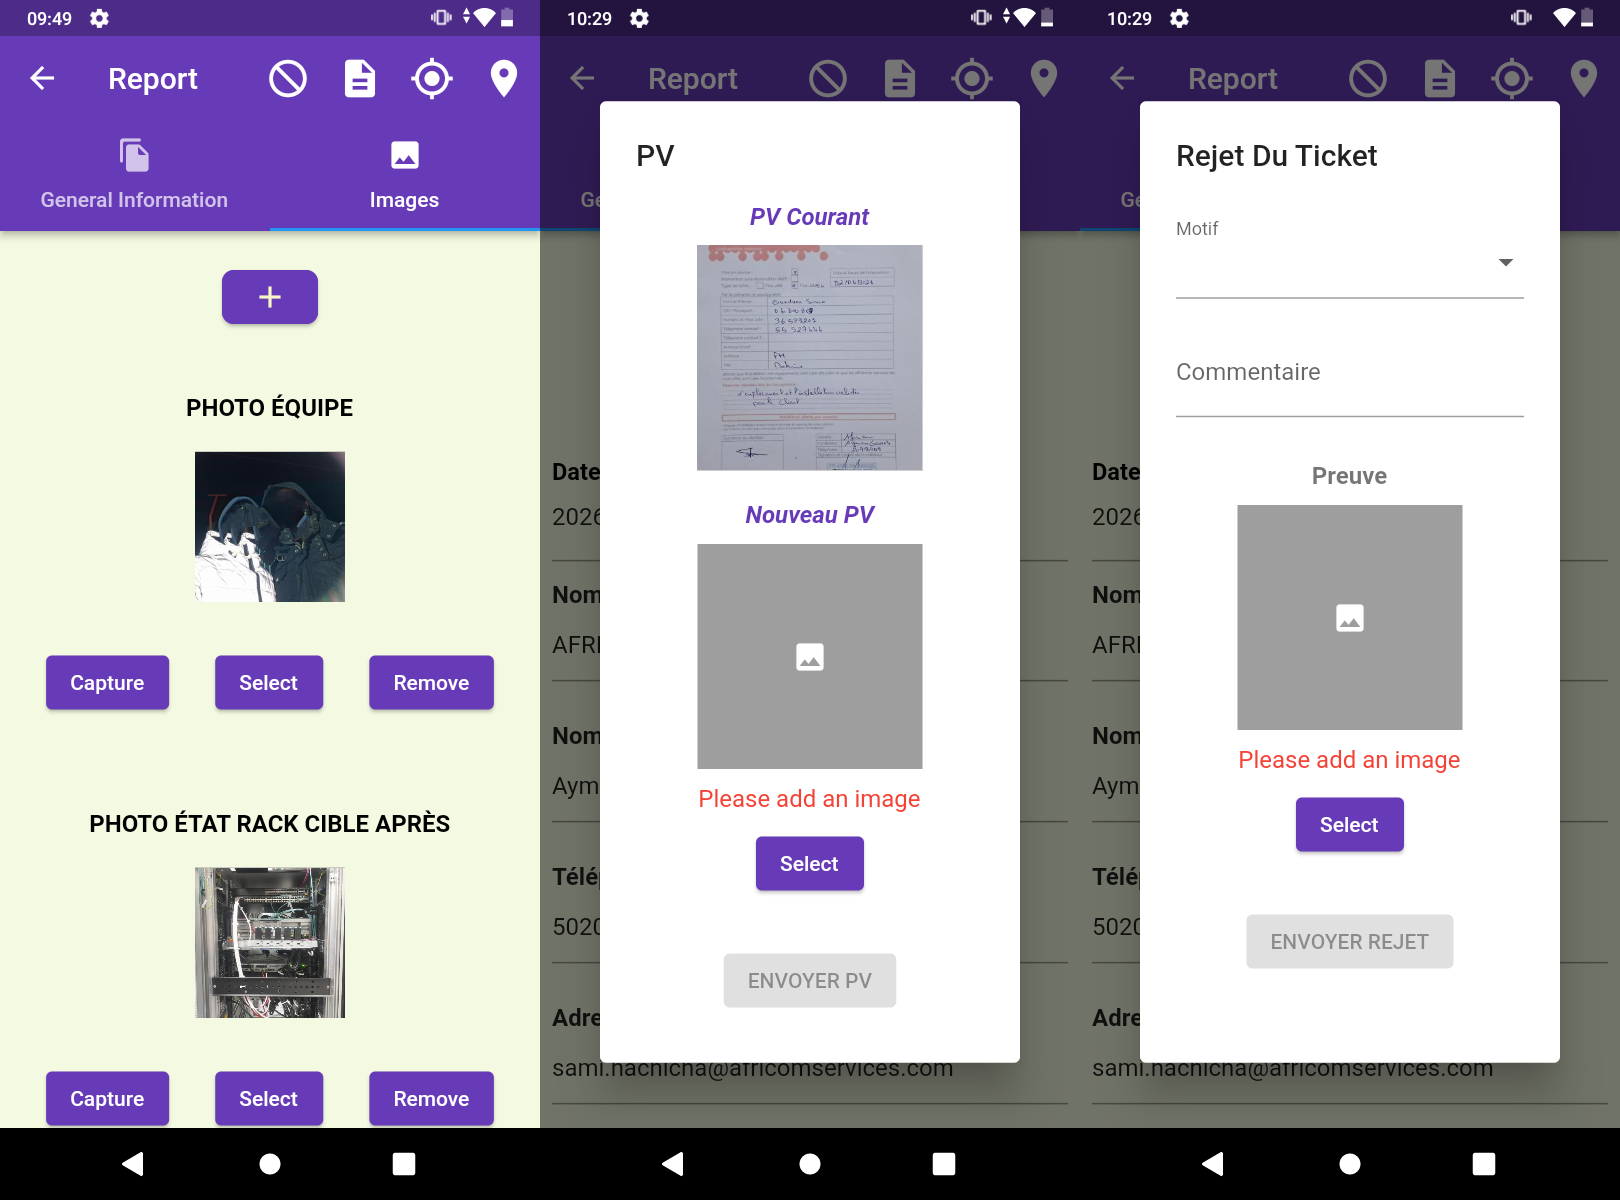
\includegraphics[width=1\textwidth]{filesFinal.png}
Flutter Mobile UI : File upload and intervention evidence capture.
}}
\caption{Sprint 3 Flutter UI - File Upload}
\label{fig:sprint3_flutter_files}
\end{figure}

\subsection{Database Design (PostgreSQL)}

Sprint 3 extended the database schema to support file storage metadata and geolocation tracking.

\begin{itemize}
\item \texttt{files} table for storing file metadata (name, type, size, path)
\item Relationship between files and intervention requests
\item \texttt{execution\_details} table for storing geolocation coordinates and timestamps
\item One-to-one association between execution details and intervention request
\end{itemize}

The database design ensures efficient storage of file references while delegating actual file content storage to the file system or external storage service. Geolocation data is structured to allow future analytics and reporting on technician movements.

\begin{figure}[H]
\centering
\fbox{\parbox{0.8\textwidth}{
\centering
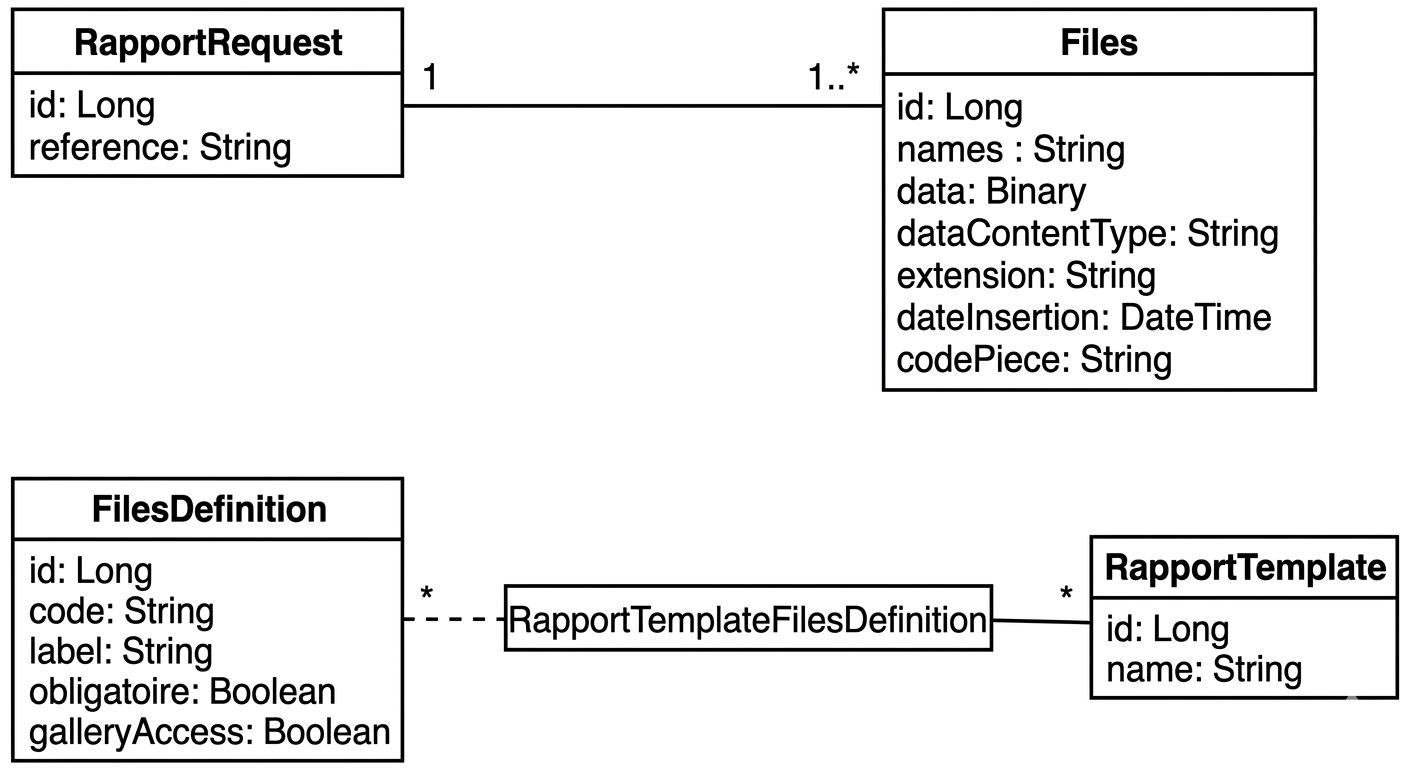
\includegraphics[width=0.8\textwidth]{dbFiles.png}
Database : File metadata
}}
\caption{Sprint 3 Database Schema}
\label{fig:sprint3_db}
\end{figure}

\subsection{API and Endpoint Summary}

\begin{table}[H]
\centering
\caption{Sprint 3 API Summary}
\label{tab:sprint3_api_summary}
\begin{tabularx}{\textwidth}{|l|l|X|}
\hline
\textbf{Method} & \textbf{Endpoint} & \textbf{Purpose} \\
\hline
POST & \api{files/upload} & Upload file and attach it to an intervention \\
\hline
GET & \api{files/{id}} & Retrieve file metadata \\
\hline
GET & \api{files/download/{id}} & Download file content securely \\
\hline
POST & \api{execution-details} & Store geolocation data for an intervention \\
\hline
GET & \api{execution-details/{requestId}} & Retrieve execution location data \\
\hline
\end{tabularx}
\end{table}

\section{Conclusion}

Sprint 3 successfully extended the system with comprehensive file management and geolocation capabilities. Technicians can now capture and upload evidence files, with automatic image compression optimizing storage while geolocation tracking provides accountability and operational insights.

Key achievements:
\begin{itemize}
\item Secure file upload and storage with access control
\item Automatic image compression and optimization
\item Mobile geolocation tracking integration
\item File download and sharing capabilities
\end{itemize}

Sprint 4 will focus on the approval workflow and status management, enabling supervisors to review and approve completed interventions.
